\documentclass{standalone}
\usepackage{tikz}
\usepackage{amsmath}
\usepackage{color}
\usetikzlibrary{matrix}
\usetikzlibrary {shapes.geometric}

\begin{document}
    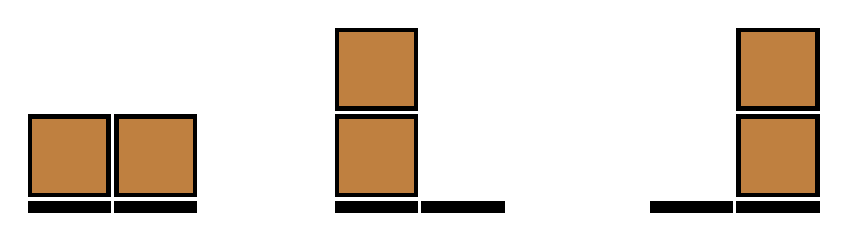
\begin{tikzpicture}
        % \draw [help lines] (0,0) grid (15,15);

        \draw [fill=brown, ultra thick] (6.2,0) rectangle (7.2,1);
        \draw [fill=black, ultra thick] (6.2,-0.1) rectangle (7.2,-0.2);
        \draw [fill=black, ultra thick] (5.1,-0.1) rectangle (6.1,-0.2);
        \draw [fill=brown, ultra thick] (5.1,0) rectangle (6.1,1);

        \draw [fill=brown, ultra thick] (9,0) rectangle (10,1);
        \draw [fill=brown, ultra thick] (9,1.1) rectangle (10,2.1);
        \draw [fill=black, ultra thick] (9,-0.1) rectangle (10,-0.2);
        \draw [fill=black, ultra thick] (10.1,-0.1) rectangle (11.1,-0.2);
        \draw [fill=black, ultra thick] (13,-0.1) rectangle (14,-0.2);
        \draw [fill=black, ultra thick] (14.1,-0.1) rectangle (15.1,-0.2);
        \draw [fill=brown, ultra thick] (14.1,0) rectangle (15.1,1);
        \draw [fill=brown, ultra thick] (14.1,1.1) rectangle (15.1,2.1);
    \end{tikzpicture}
    
\end{document}